% \VignetteIndexEntry{An R Package for sendplot}
% \VignetteDepends{sendplot}
% \VignetteKeyword{sendplot}
% \VignetteKeyword{sendplotVignette}

\documentclass[]{article}

\title{sendplot}
\author{Lori Shepherd}

\usepackage{/projects/aCGH/Active/CodeDevelopment/R/lib/R/share/texmf/Sweave}
\begin{document}

\maketitle

\quad sendplot creates an interactive plot with any number of decoration plots also being displayed. Although the creation of these files must be in R, R is not required for viewing output. The necessary elements for viewing an interactive plot is a web browser that has javascript capabilities. The code used to create this is a modified version of the javascript code from \\
http://www.onlamp.com/pub/a/onlamp/2007/07/05/writing-advanced-javascript.html \\
or it utilizes an open source tooltip library called wz\_tooltip.js from \\
 http://www.walterzorn.com/tooltip/tooltip\_e.htm
Note if you are using Internet Explorer you may need to select the option allowed bloced content. Internet Explorer will initially block the scripts from running. A warning message normally appears towards the top of the browser; if you click on this warning it will give an option to allow blocked content. 
\quad We will now go through an example of running this application. This example is a more advanced usage; for basic examples please see the R help files for sendplot, sendxy or sendimage; sendxy and sendimage are wrappers to the sendplot function that will create a single interactive scatterplot or image plot. We will go through the steps to make Figure 1 where the main image heatmap is interactive.

\begin{center}
\begin{figure}
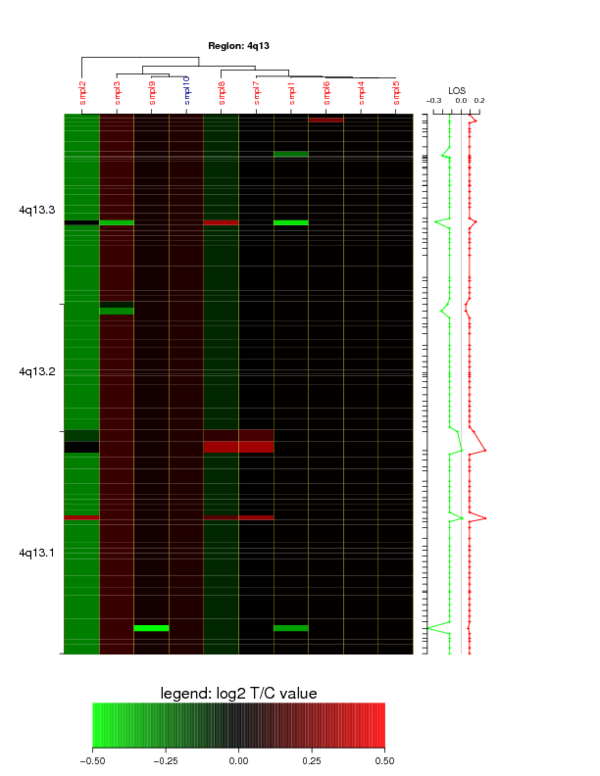
\includegraphics{test}
\caption{Interactive heatmap image}
\end{figure}
\end{center}

Begin by cleaning the workspace and loading the library. This example utilizes objects created with the R package aCGHplus. aCGHplus is a package designed for array comparative genomic hybridization experiments. For information on this package and objects that can be created with this package please go to the website: http://sphhp.buffalo.edu/biostat/research/software/acghplus/index.php. We load the aCGH object as well:

\begin{Schunk}
\begin{Sinput}
> rm(list = ls())
> library(sendplot)
> data("aCGHex")
\end{Sinput}
\end{Schunk}
Lets look at each argument of the sendplot function call. As a reminder the sendplot function is:
\begin{verbatim}
sendplot <- function(mat, plot.calls, x,y, mai.mat, mai.prc=FALSE,xlim=NA, ylim=NA,
                     z=NA, z.value="value",type="scatterplot", plt.extras = NA,
                     x.lbls=NA, y.lbls=NA, xy.lbls=NA,
                     bound.pt = TRUE,source.plot=NA,resize="4000x5500", ps.paper="letter",
                     ps.width=8,ps.height=11,fname.root="test",dir="./",header="v2",
                     paint=TRUE,  img.prog = NA,
                     up.left=c(673,715),low.right=c(2874,4481),
                     spot.radius=10
                     )
\end{verbatim}
\quad The first argument, mat, is a numeric matrix that will be passed in the R graphics package function layout. In this case we will set up a display for four different plots.

\begin{Schunk}
\begin{Sinput}
> mat = matrix(c(rep(c(rep(2, 8), rep(0, 2)), 1), rep(c(rep(1, 
+     8), rep(4, 2)), 14), rep(c(rep(3, 8), rep(0, 2)), 2)), ncol = 10, 
+     byrow = TRUE)
\end{Sinput}
\end{Schunk}
The layout that will be used is:
\begin{Schunk}
\begin{Soutput}
      [,1] [,2] [,3] [,4] [,5] [,6] [,7] [,8] [,9] [,10]
 [1,]    2    2    2    2    2    2    2    2    0     0
 [2,]    1    1    1    1    1    1    1    1    4     4
 [3,]    1    1    1    1    1    1    1    1    4     4
 [4,]    1    1    1    1    1    1    1    1    4     4
 [5,]    1    1    1    1    1    1    1    1    4     4
 [6,]    1    1    1    1    1    1    1    1    4     4
 [7,]    1    1    1    1    1    1    1    1    4     4
 [8,]    1    1    1    1    1    1    1    1    4     4
 [9,]    1    1    1    1    1    1    1    1    4     4
[10,]    1    1    1    1    1    1    1    1    4     4
[11,]    1    1    1    1    1    1    1    1    4     4
[12,]    1    1    1    1    1    1    1    1    4     4
[13,]    1    1    1    1    1    1    1    1    4     4
[14,]    1    1    1    1    1    1    1    1    4     4
[15,]    1    1    1    1    1    1    1    1    4     4
[16,]    3    3    3    3    3    3    3    3    0     0
[17,]    3    3    3    3    3    3    3    3    0     0
\end{Soutput}
\end{Schunk}
\quad The numbers 1-4 represent the areas that will contain four different plots. The first plot displaying in the region marked as one, the second in the region marked as two, and so on. In our final display, the first and fourth plot line up. For this reason there is a buffer region of 0 above and below the fourth plot. Zero acts as a region that no graph is displayed. \\

\quad The next argument, plot.calls, is a character vector with the necessary plot calls for all graphs. In this example plot.calls will be of length four. The call that is included is the main chunk of the plot call or the main shell of what is plotted. Additional expressions can be evaluated on the plot through the sendplot argument plt.extras. For example, you may want to graph an image as the main plot call but you may want to specify a particular axis or tick marks. The image call goes into plot.calls while an axis call goes into the plt.extras argument. We will look at plt.extras in more detail momentarily. The plot.calls argument for Figure 1 is:

\begin{verbatim}
plot.calls = c(
     "image(x=x,y=y,z=t(z),zlim=c(-0.5,0.5), ylim=range(scanLoc,na.rm=T),
            col=c(hsv(h=2/6,v=seq(1,0,length=1000)^1.15),
            hsv(h=0/6,v=seq(0,1,length=1000)^1.15)),axes=F,xlab='',ylab='')",

     "plot(ddr,axes = FALSE, xaxs = 'i', leaflab = 'none',main=ttl)",

     "image(x=seq(from=-0.5,to=0.5,length=1000),y=1,z=t(zlgnd),zlim=c(-0.5,0.5),
            col=c(hsv(h=2/6,v=seq(1,0,length=1000)^1.15),
                  hsv(h=0/6,v=seq(0,1,length=1000)^1.15)),
            axes=F,xlab='',ylab='')",

     "image(x=0:1,y=0:1,z=matrix(rep(NA,4),ncol=2),xlim=range(c(W.lw,W.up),na.rm=T),
            ylim=range(scanLoc,na.rm=T),zlim=c(0,1),axes=F,xlab='',ylab='')")

\end{verbatim}

The first plot call, 
\begin{verbatim}
"image(x=x,y=y,z=t(z),zlim=c(-0.5,0.5), ylim=range(scanLoc,na.rm=T),
            col=c(hsv(h=2/6,v=seq(1,0,length=1000)^1.15),
            hsv(h=0/6,v=seq(0,1,length=1000)^1.15)),axes=F,xlab='',ylab='')",
\end{verbatim}
creates a heatmap image that looks like Figure 2. Notice axis and additional plotting such as vertical line breaks have not yet been plotted.  
\begin{center}
\begin{figure}
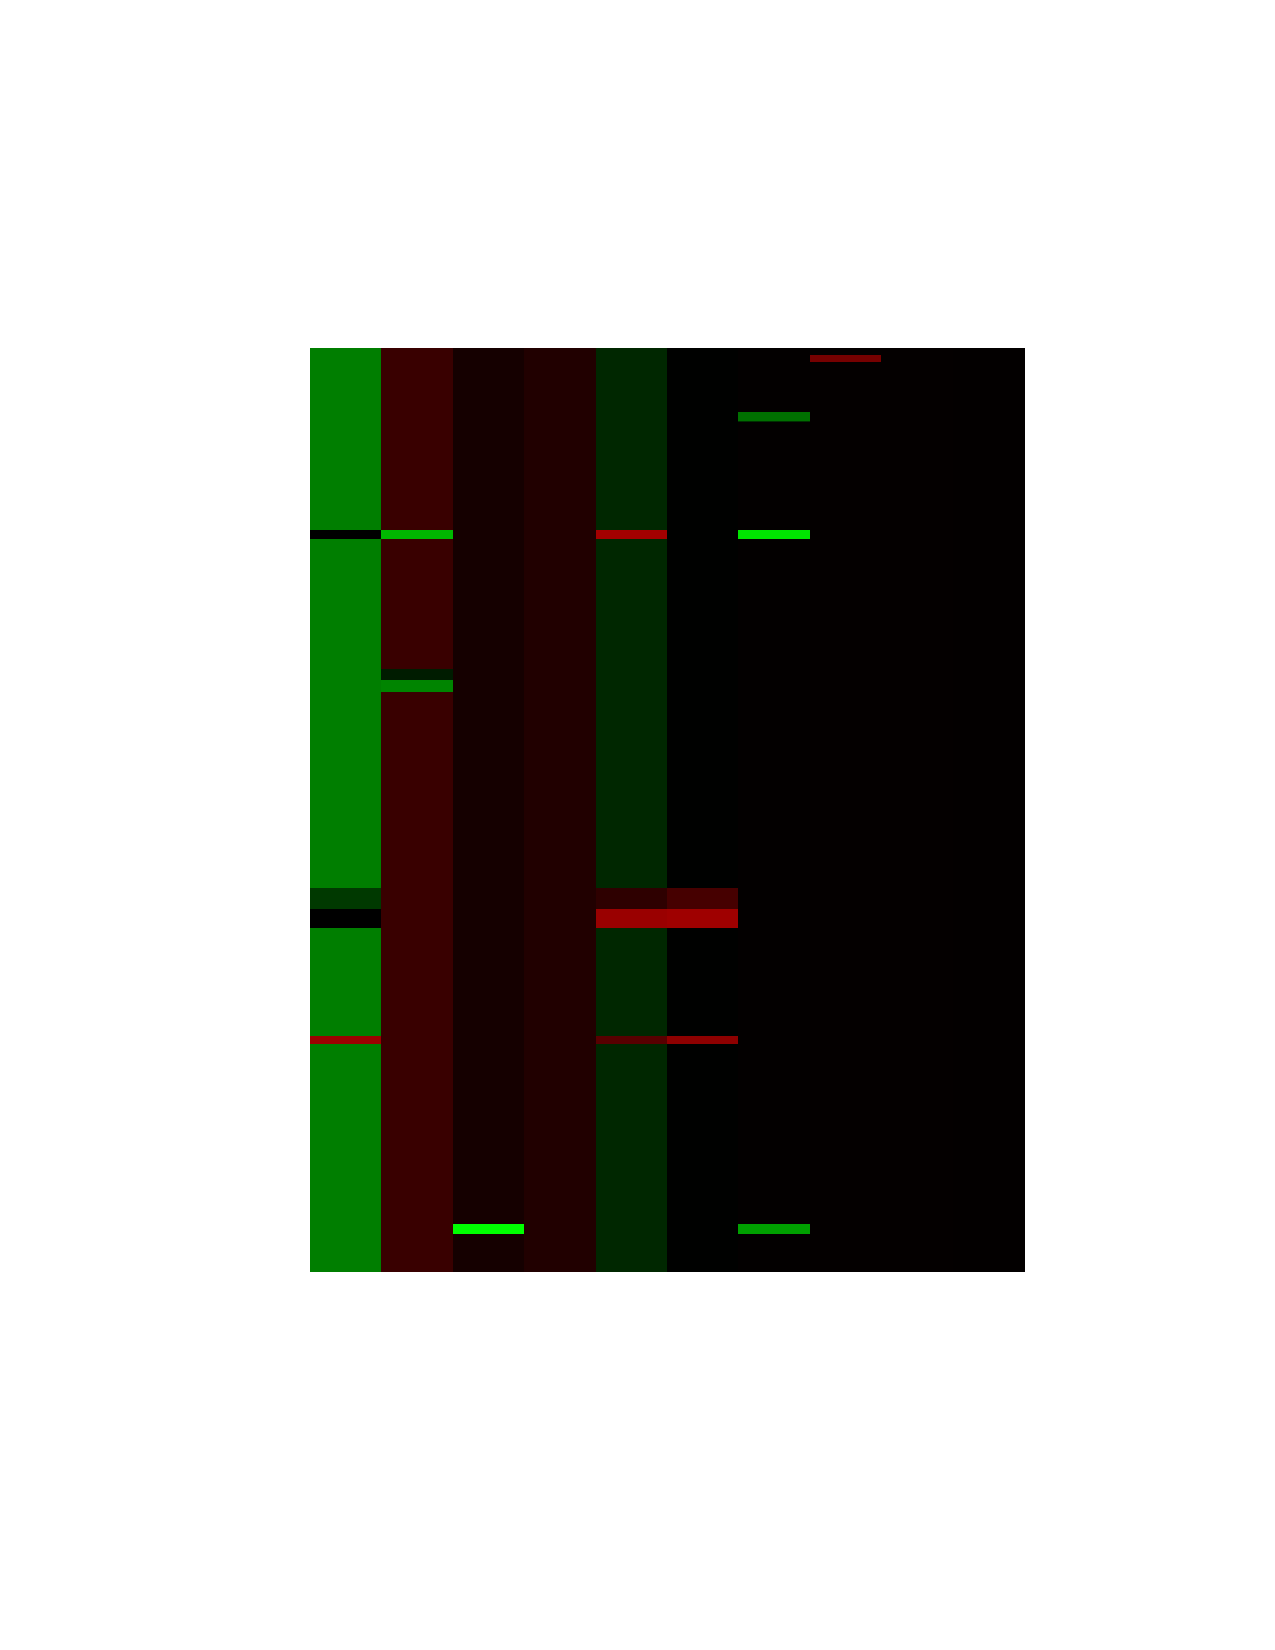
\includegraphics[scale=.5]{heatmap}
\caption{Initial heatmap image from executing plot.call[1]}
\end{figure}
\end{center}

The second plot call, 
\begin{verbatim}
plot(ddr,axes = FALSE, xaxs = 'i', leaflab = 'none',main=ttl)
\end{verbatim}
creates the dendrogram representation of sample clustering seen in Figure 3. 
\begin{center}
\begin{figure}
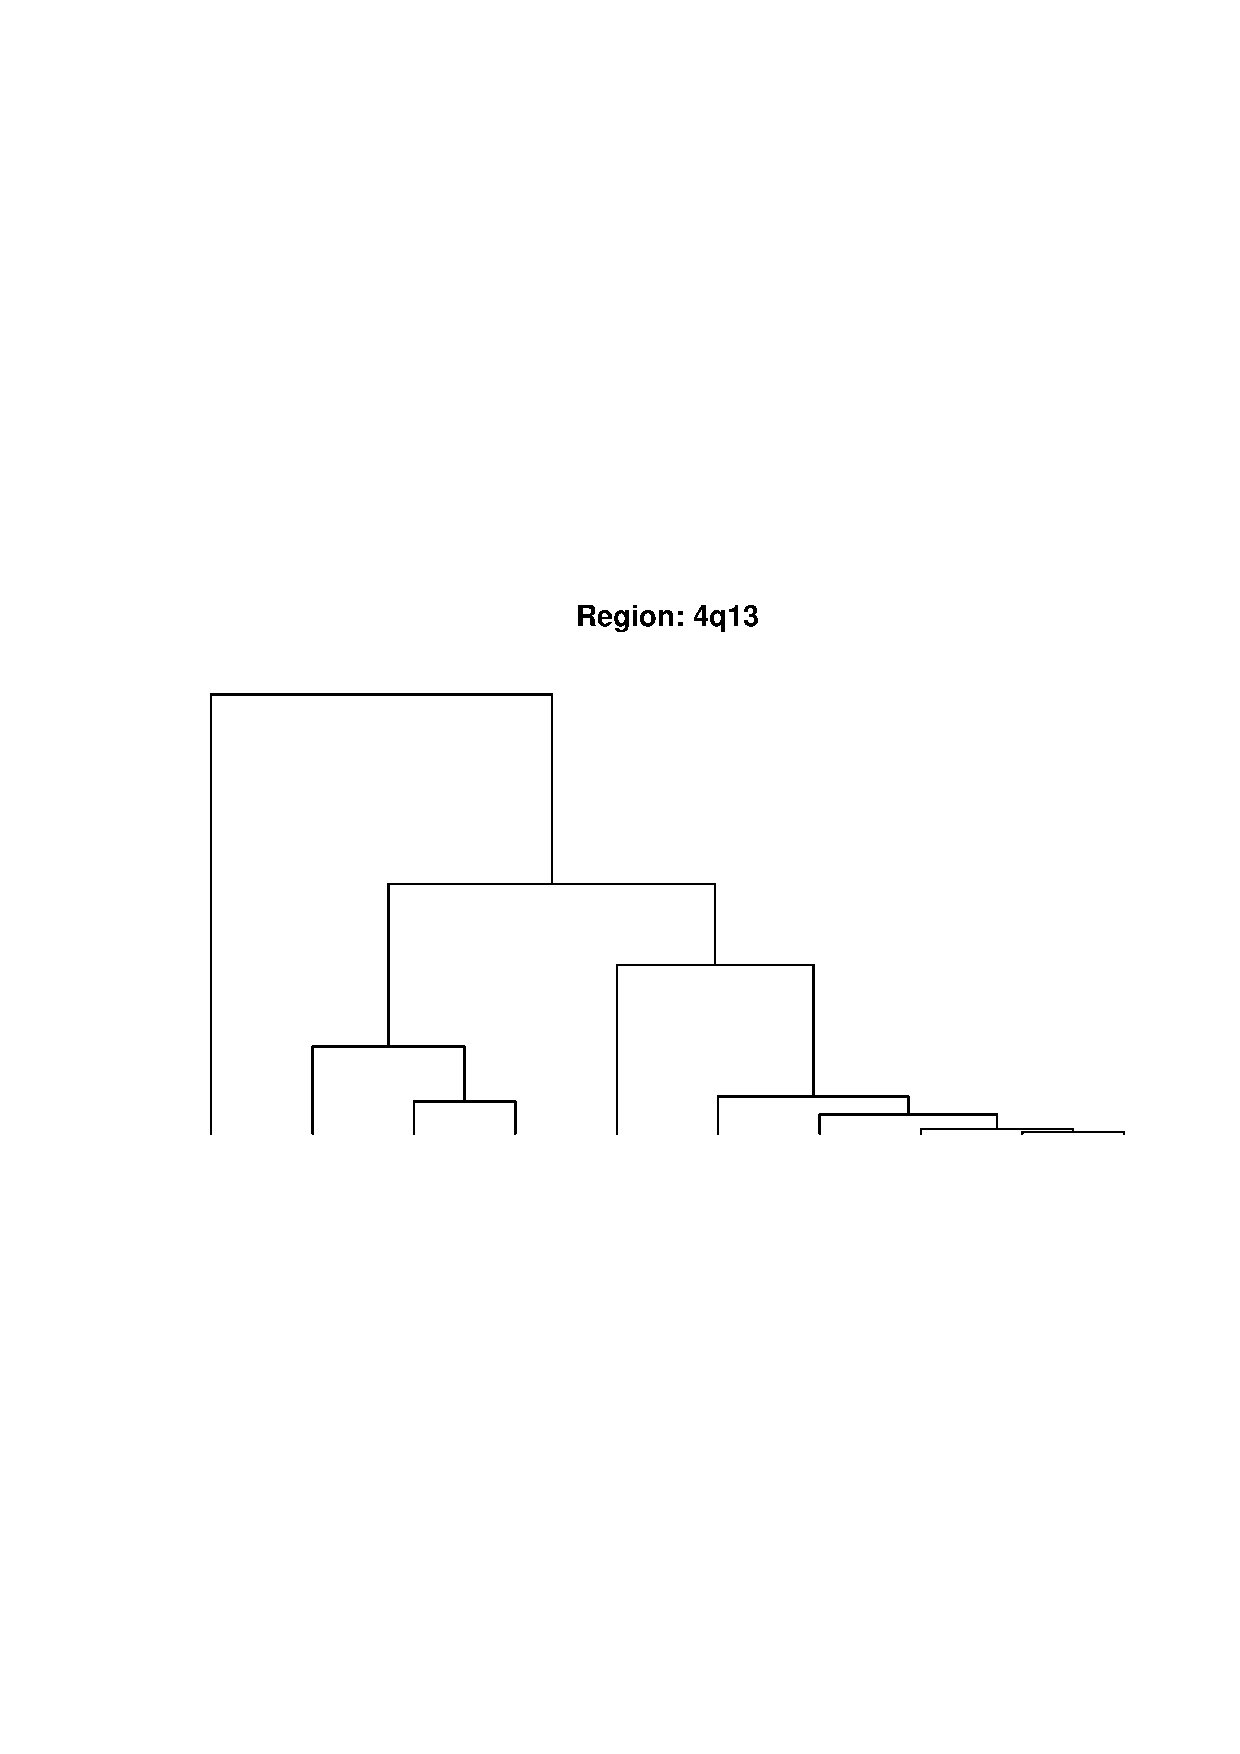
\includegraphics{dendro}
\caption{Dendrogram created from executing plot.call[2]}
\end{figure}
\end{center}

The third plot call, 
\begin{verbatim}
  image(x=seq(from=-0.5,to=0.5,length=1000),y=1,z=t(zlgnd),zlim=c(-0.5,0.5),
        col=c(hsv(h=2/6,v=seq(1,0,length=1000)^1.15),
        hsv(h=0/6,v=seq(0,1,length=1000)^1.15)),
        axes=F,xlab='',ylab='')
\end{verbatim}
creates the legend image seen in Figure 4. 
\begin{center}
\begin{figure}

\includegraphics{legend}
\caption{Legend created from executing plot.call[3]}
\end{figure}
\end{center}

The last plot.call, 
\begin{verbatim}
image(x=0:1,y=0:1,z=matrix(rep(NA,4),ncol=2),
        xlim=range(c(W.lw,W.up),na.rm=T),
        ylim=range(scanLoc,na.rm=T),
        zlim=c(0,1),
        axes=F,xlab='',ylab='')
\end{verbatim}
creates a blank image. We choose to use image as a base instead of plot to ensure ratios and buffers would be equivalent between the first and fourth plots.
\\
\quad There are many features that have not been included with the main plot calls in the plot.calls argument. These will be added by the plt.extras argument. If you look closely at the plot calls, you will notice that they use many variables we have yet to define. Any variables that are used in plotting calls should be in local R memory at the time of execution. The following are variables needed for plot calls:
\begin{verbatim}
# index of genome - we want to look at region 4q13 
# the aCGHplus object has already been subset for this region for 10 samples
   scanDX = 1:dim(aCGH$mapping.info)[1]
   bioDX = scanDX
   scanLoc=aCGH$mapping.info$loc.genome[scanDX]
   scanLoc[which(diff(scanLoc)<=0)]=scanLoc[which(diff(scanLoc)<=0)]-0.001
# add sample names to index of log2 data
   colnames(aCGH$log2.ratios.fitted)=aCGH$inventory$sample.ID
# perform a sample clustering and create dendrogram 
   ManDist=dist(t(aCGH$log2.ratios.fitted),method = "manhattan")
   hc=hclust(ManDist,method="ward")
   ddr=as.dendrogram(hc)
# useful sample information
   nsmpl = aCGH$data.info$nsmpl
   smplDX = 1:nsmpl
   ttl = "Region: 4q13"
# creates legend scale for log2 ratios from -.5 to .5
   zlgnd=array(seq(from=-0.5,to=0.5,length=1000),dim=c(1,1000))
# x values = samples 
   x = 1:length(smplDX)
# y values = genomic location
   y = scanLoc
# z values = log 2 ratios that have been fitted 
# by circulary binay segmentation - min and max cutoffs applied
   z.value="log2.ratios.fitted"
   z = aCGH$log2.ratios.fitted[,hc$order]
   z.raw = z
   z[z>0.5]=0.5
   z[z<(-0.5)]=-0.5
# sorts log2 values and splits into low region and high region
# to create fourth plot of avg. means 
   rowSort=function(i,x) sort(x[i,])
   z.sort=t(mapply(rowSort,1:(dim(z.raw)[1]),MoreArgs=list(x=z.raw)))
   lwDX=1:ceiling(nsmpl/4)
   upDX=(floor((3/4)*nsmpl)+1):nsmpl
   W.up=rowMeans(z.sort[,upDX],na.rm=T)
   W.lw=rowMeans(z.sort[,lwDX],na.rm=T)
\end{verbatim}

\quad We now return to the arguments of sendplot. We have defined the mat and the plot.calls arguments for our example. The next argument is mai.mat. This perhaps is the hardest for a user to define. mai.mat is a matrix that holds the arguments for each plots' margins. Each row is a different mai vector. These values will be passed into the R graphics package par(mai=) command. The matrix is n by four, where n is the number of plot calls. The four columns represent the margins bottom, left, top, and right as defined by the R graphics pagkage function par. If the figure margins are set too large an error will occur when plotting. If the user gets an Error figure margins too large, decrease the values in mai.mat.The mai.mat for our example is created with the following code:

\begin{Schunk}
\begin{Sinput}
> mai.mat = matrix(0, ncol = 4, nrow = 4, byrow = TRUE)
> mai.mat[1, ] = c(0.5, 0, 0.5, 0)
> mai.mat[2, ] = c(0, 0, 0.3, 0)
> mai.mat[3, ] = c(0.4, 0.4, 0.2, 0.4)
> mai.mat[4, ] = c(0.5, 0.2, 0.5, 0.2)
\end{Sinput}
\end{Schunk}
\quad The first row, mai.mat[1,], indicates the figure margins for the first plot. The heatmap plot will have a bottom and top margin of .5, while the left and right will have no margin.The second row, mai.mat[2,], indicates the figure margins for the second plot. The dendrogram plot will have no left or right margin so that it will line up with the heatmap width, no bottom margin, but a top margin of .3. The  others follow accordingly.  The mai.mat values may also be a percentage of the default margins rather than hard coded values. If the values in mai.mat are percentages an argument mai.prc should be tripped to TRUE.\\


\quad The x, y, and z arguments of the sendplot function have already been defined. The x argument is the x values that will be used for graphing the first plot. The y argument is the y values that will be used for graphing the first plot. These need to be specified again seperatly from the plot calls in order to accurately make the first plot's points interactive. If the first plot is an image, the z argument is the z values used in the first plot's image call. If the first plot is a scatterplot z will be left as NA. We have already defined x, y, and z in local memory. z.value is the label for what is being displayed by the z values. This label will be used in the interactive window display. It should not contain any spaces. The data being used as z values for our example is log2 ratios that have been fitted by circular binary segmentation. We will call our z.value log2ratios.fitted.

\begin{Schunk}
\begin{Sinput}
> z.value = "log2ratios.fitted"
> xlim = NA
> ylim = NA
> type = "image"
\end{Sinput}
\end{Schunk}
\quad In the above code we have set three more of the sendplot function's arguments: xlim, ylim, and type. xlim and ylim only need to be specified if the type is scatterplot. xlim and ylim help define the range of the data for accurate display of information when the points of a scatterplot are interactive. The xlim and ylim should be defined as the appropriate minimum and maximum value to use for the plot axis. If the type is scatterplot and the xlim or ylim is left as NA, the range of the x values and range of y values are used. Our example is a heatmap which is plotted by image. xlim and ylim therefore remain NA. The xlim and ylim values will be generated from the image call. Type indicates the type of graph that the first, main plot of the plot.calls is. Currently supported types are scatterplot or image. Our first plot is generated with an image call, and therefore is of type image.  

\quad We now return to the plt.extras argument. plt.extras is a list of length equal to the number of plot.calls. In our example, plt.extras should be of length four. Each argument of the list is also a list, which we will refer to as a sublist. Each sublist contains character vectors with additional plot calls for the plot created with the plot.call of the location of the sublist in the plt.extras. For example, the sublist test has two calls and we want them to be graphed on the second plot or plot.calls[2] while there are no additional plot calls for the first plot:

\begin{verbatim}
plt.extras = list()
plt.extras$plot1 = NA
test = list()
test[1] = "abline(v=0, col='gray77', lwd=1)"
test[2] = "title(main='mytest')"
plt.extras$plot2 = test
\end{verbatim}  


\quad If we look back at Figure 2 compared with Figure 1, we see we want to add an axis to the left and top of the plot with labels, and vertical lines to seperate x values. The following code will achieve this:  
\begin{verbatim}
plot1 = list()
plt1.ind = 1

nlbl=50
eval.js("sample.colors=as.character(aCGH$inventory$sex)")
colorSet =c("hotpink","darkblue", "green")
lev = levels(factor(sample.colors))
for(i in 1:length(lev)){
  sample.colors[sample.colors==lev[i]] = colorSet[i]
}
count.arm=sum((aCGH$Band.Aid$Regions[[2]]$Upper>=min(scanLoc,na.rm=T))
  &(aCGH$Band.Aid$Regions[[2]]$Lower<=max(scanLoc,na.rm=T)))
count.broadband=sum((aCGH$Band.Aid$Regions[[3]]$Upper>=min(scanLoc,na.rm=T))
  &(aCGH$Band.Aid$Regions[[3]]$Lower<=max(scanLoc,na.rm=T)))
count.finband=sum((aCGH$Band.Aid$Regions[[4]]$Upper>=min(scanLoc,na.rm=T))
  &(aCGH$Band.Aid$Regions[[4]]$Lower<=max(scanLoc,na.rm=T)))
cat("label counts:",count.arm,count.broadband,count.finband,fill=T)
cat("target number=",nlbl,fill=T)
ilbl=order(abs(c(count.arm,count.broadband,count.finband,length(scanDX))-nlbl))[1]
cat("ilbl=",ilbl,fill=T)
if(ilbl<=3){
  if(ilbl==1) bandDX=1:40
  if(ilbl==2) bandDX=(
       (sum(aCGH$Band.Aid$Regions[[3]]$Upper<=min(scanLoc,na.rm=T),na.rm=T)+1)
       :(sum(aCGH$Band.Aid$Regions[[3]]$Lower<=max(scanLoc,na.rm=T),na.rm=T)))
  if(ilbl==3) bandDX=(
       (sum(aCGH$Band.Aid$Regions[[4]]$Upper<=min(scanLoc,na.rm=T),na.rm=T)+1)
       :(sum(aCGH$Band.Aid$Regions[[4]]$Lower<=max(scanLoc,na.rm=T),na.rm=T)))
  lbls=paste(aCGH$Band.Aid$Regions[[ilbl+1]]$Chrom[bandDX],
    aCGH$Band.Aid$Regions[[ilbl+1]]$Label[bandDX],sep="")


  plot1[plt1.ind] =  "axis(2,aCGH$Band.Aid$Regions[[ilbl+1]]$Center[bandDX],
                           tick=F,labels=lbls,las=2,cex.axis=1)"
  plt1.ind = plt1.ind +1 
  plot1[plt1.ind] = "axis(2,aCGH$Band.Aid$Regions[[ilbl+1]]$Lower[bandDX], labels=F)"
  plt1.ind = plt1.ind +1 
  
}
if(ilbl==4){   
  lbls=as.character(aCGH$mapping.info$spot.ID[scanDX])

  plot1[plt1.ind] = "axis(2,aCGH$mapping.info$loc.genome[scanDX],tick=F,
          labels=lbls, las=2,cex.axis=1)"
  plt1.ind = plt1.ind +1 
}

plot1[plt1.ind] = "abline(v=(0:nsmpl)+1/2,col=7,lty=1,lwd=1/3)"
plt1.ind = plt1.ind +1


if(length(sample.colors)==1){

  plot1[plt1.ind] = "axis(3,1:length(smplDX),cex.axis=1,las=2,
                     labels=aCGHsub$inventory$sample.ID[hc$order])"
  plt1.ind = plt1.ind +1 
}                                      
if(length(sample.colors)!=1){
  unq.colors=unique(sample.colors[hc$order])
  lbls2=aCGH$inventory$sample.ID[hc$order]
  col.labs=sample.colors[hc$order]
  for(j in 1:length(unq.colors)){
    iclr = unq.colors[j]
    cat("eye color=",iclr,fill=T)
    nm = paste("adx",j,sep="")
    eval.js(paste(nm, "=which(col.labs==iclr)",sep=""))

    plot1[plt1.ind] = paste("axis(3,",nm,",labels=lbls2[",nm,"],
                      cex.axis=1,las=2,col.axis='",iclr,"')", sep="")
    plt1.ind = plt1.ind +1 
  }     
}
\end{verbatim}

\quad The second plot of the dendrogram does not require any additional plotting and therefore will be NA. The legend created by the third plot call requires a title and a bottom axis. This will be achieved by setting up the following:

\begin{Schunk}
\begin{Sinput}
> plot3 = list()
> plt3.ind = 1
> plot3[plt3.ind] = "mtext('legend: log2 T/C value',side=3,cex=1,line=1/4)"
> plt3.ind = plt3.ind + 1
> plot3[plt3.ind] = "axis(1,seq(from=-0.5,to=0.5,length=5),line=0)"
> plt3.ind = plt3.ind + 1
\end{Sinput}
\end{Schunk}
\quad The entire fourth graph still needs to be generated since we only set up an image shell. The following calls will achieve this:

\begin{Schunk}
\begin{Sinput}
> plot4 = list()
> plt4.ind = 1
> plot4[plt4.ind] = "abline(v=0,col='gray77',lwd=1)"
> plt4.ind = plt4.ind + 1
> plot4[plt4.ind] = "points(W.lw,scanLoc,col='green',pch=3,cex=0.5)"
> plt4.ind = plt4.ind + 1
> plot4[plt4.ind] = "points(W.up,scanLoc,col='red',pch=3,cex=0.5)"
> plt4.ind = plt4.ind + 1
> plot4[plt4.ind] = "lines(W.lw,scanLoc,col='green',pch=3,cex=0.5)"
> plt4.ind = plt4.ind + 1
> plot4[plt4.ind] = "lines(W.up,scanLoc,col='red',pch=3,cex=0.5)"
> plt4.ind = plt4.ind + 1
> plot4[plt4.ind] = "axis(3)"
> plt4.ind = plt4.ind + 1
> plot4[plt4.ind] = "mtext(text='LOS',side=3,line=2,cex=0.5)"
> plt4.ind = plt4.ind + 1
> plot4[plt4.ind] = "axis(2,at=scanLoc,labels=F)"
> plt4.ind = plt4.ind + 1
\end{Sinput}
\end{Schunk}
\quad The above code generates all the sublists of the plt.extras list. The following will put all the sublists in the plt.extras list object:

\begin{Schunk}
\begin{Sinput}
> plt.extras = list()
> plt.extras$plot1 = plot1
> plt.extras$plot2 = NA
> plt.extras$plot3 = plot3
> plt.extras$plot4 = plot4
\end{Sinput}
\end{Schunk}
\quad The plt.extras argument has now been generated for our example. Notice how this argument will add any additional plot calls to the original plot. Our plt.extras is of length four which is consistant with the length of our plot.calls argument. The sublist for the first plot of the heatmap image, plot1, has five additional plot arguments: one call generating vertical lines at all x boundaries, two calls generating axis, one for the top and one for the left, and two calls generating tick labels for the axis.
\begin{Schunk}
\begin{Sinput}
> plot1
\end{Sinput}
\begin{Soutput}
[[1]]
[1] "axis(2,aCGH$Band.Aid$Regions[[ilbl+1]]$Center[bandDX],tick=F,labels=lbls,las=2,cex.axis=1)"

[[2]]
[1] "axis(2,aCGH$Band.Aid$Regions[[ilbl+1]]$Lower[bandDX], labels=F)"

[[3]]
[1] "abline(v=(0:nsmpl)+1/2,col=7,lty=1,lwd=1/3)"

[[4]]
[1] "axis(3,adx1,labels=lbls2[adx1],cex.axis=1,las=2,col.axis='hotpink')"

[[5]]
[1] "axis(3,adx2,labels=lbls2[adx2],cex.axis=1,las=2,col.axis='darkblue')"
\end{Soutput}
\end{Schunk}
 The sublist for the second plot of the dendrogram, plot2, is NA because there is no additional graphing needed. The legend is the third plot, plot3, which has two additional calls: one to make the title of the image and one to make the axis. 
\begin{Schunk}
\begin{Sinput}
> plot3
\end{Sinput}
\begin{Soutput}
[[1]]
[1] "mtext('legend: log2 T/C value',side=3,cex=1,line=1/4)"

[[2]]
[1] "axis(1,seq(from=-0.5,to=0.5,length=5),line=0)"
\end{Soutput}
\end{Schunk}
The fourth plot consists of eight different additional plotting calls which make axis, add labels, and add points and lines.   

\begin{Schunk}
\begin{Sinput}
> plot4
\end{Sinput}
\begin{Soutput}
[[1]]
[1] "abline(v=0,col='gray77',lwd=1)"

[[2]]
[1] "points(W.lw,scanLoc,col='green',pch=3,cex=0.5)"

[[3]]
[1] "points(W.up,scanLoc,col='red',pch=3,cex=0.5)"

[[4]]
[1] "lines(W.lw,scanLoc,col='green',pch=3,cex=0.5)"

[[5]]
[1] "lines(W.up,scanLoc,col='red',pch=3,cex=0.5)"

[[6]]
[1] "axis(3)"

[[7]]
[1] "mtext(text='LOS',side=3,line=2,cex=0.5)"

[[8]]
[1] "axis(2,at=scanLoc,labels=F)"
\end{Soutput}
\end{Schunk}
\quad It is worth noting that some of the plt.extras arguments can be included in the plot.calls argument. This is achieved by seperating any calls for the same plot with a semicolon. For example, the third plot.call for the heatmap legend, originally is  
\begin{verbatim}
"image(x=seq(from=-0.5,to=0.5,length=1000),y=1,z=t(zlgnd),zlim=c(-0.5,0.5),
            col=c(hsv(h=2/6,v=seq(1,0,length=1000)^1.15),
                  hsv(h=0/6,v=seq(0,1,length=1000)^1.15)),
            axes=F,xlab='',ylab='')",
\end{verbatim}
and the plt.extras calls were 
\begin{verbatim}
  "mtext('legend: log2 T/C value',side=3,cex=1,line=1/4)"
  
   and 

   "axis(1,seq(from=-0.5,to=0.5,length=5),line=0)"
\end{verbatim}

\quad We could have placed both of the plt.extra calls in the plot.calls argument and changed the plt.extra call to NA. The plot.call for the third graph would become the following:
\begin{verbatim}
"image(x=seq(from=-0.5,to=0.5,length=1000),y=1,z=t(zlgnd),zlim=c(-0.5,0.5),
            col=c(hsv(h=2/6,v=seq(1,0,length=1000)^1.15),
                  hsv(h=0/6,v=seq(0,1,length=1000)^1.15)),
            axes=F,xlab='',ylab=''); mtext('legend: log2 T/C value',side=3,cex=1,line=1/4);
            axis(1,seq(from=-0.5,to=0.5,length=5),line=0)"
\end{verbatim}
\quad Notice how the three seperate calls are seperated by a semicolon but are all considered part of the first plot.call because of the placement of the quotation markers. Either is acceptable but we wanted the user to recognize this option. 

\quad The next few arguments, x.lbls, y.lbls, and xy.lbls, control what is displayed in the interactive window when the user hovers the mouse over points or regions of the first, main, plot. x.lbls refers to data that is specific to the x value of the data point or region in questions, likewise y.lbs refers to the data that is specific to the y value of the data point or region in question. xy.lbls refers to data that is specific to both x and y location. In the case of a scatterplot, x.lbls, y.lbls, and xy.lbls refer to the same position; it therefore is only necessary to use either x.lbls or y.lbls. x.lbls and y.lbls are data.frames. x.lbls is of the dimension n by m where n is equal to the length of x. Each row of the x.lbl is specific to a certain x.value. The row should be ordered to correspond with the order of the graph. Each column of the data frame is a unique piece of data. The names of the columns will be used as the label in the interactive display window. In our example x values are samples. We have 43 x values and therefore 43 rows in the x.lbls data.frame. We wish to display the information for sample.ID and sex which are sample specific data. The aCGH object contains a data.frame that holds information about the samples: the first column of that data frame holds the sample.ID information and the eighth column holds the sex data. Earlier we ordered the samples by clustering. The x.lbls data frame therefore may be attained with the following:

\begin{Schunk}
\begin{Sinput}
> x.lbls = aCGH$inventory[hc$order, c(1, 8)]
> y.lbls = aCGH$mapping.info[scanDX, c(5, 6, 8, 10, 12)]
\end{Sinput}
\end{Schunk}
\quad In our example the y values are BACs of specific genomic location. We selected a specific range of BACs by setting scanDX. There are 98 different y value locations and therefore y.lbls will have 98 rows. The y.lbls data frame is smilar to the x.lbls data frame in that it is of the dimension n by m where n is equal to the length of y. Each row of the y.lbl is specific to a certain y value and the rows should be ordered to correspond with the ordering of the graph. Each column of the y.lbls data frame is a unique piece of data. We wish to display the information for genomic location, chromosome, arm, broad.band, and fine.band location in the interactive display. The aCGH object contains a data.frame that holds information about the BACs; The corresponding columns in that data.frame are 5, 6, 8. 10, and 12. \\
\quad The xy.lbls argument is a little different because it is specific to both the selected x value and y value. The xy.lbls argument is therefore a list of matricies; Each matrix is of the dimension n by m where n is equal to the length of y and m is equal to the length of x. For our example the only xy specific data we have are raw log2 ratios and the log2 ratios that have been fitted by circular binary segmentation. Since we have used the fitted log 2 ratios as the z value to create the heatmap, these values are included automatically in the interactive display. Our example therefore has one matrix in the xy.lbls list. 

\begin{Schunk}
\begin{Sinput}
> xy.lbls = list()
> log2.ratio = as.matrix(aCGH$log2.ratios[, hc$order])
> xy.lbls$log2.ratio = log2.ratio
\end{Sinput}
\end{Schunk}
\quad The source.plot argument controls what file formats are created. The interactive html file requires a .png file. There are two possible scenerios for making a png file:
the png file may be made directly, or a postscript file may be made first and then converted into a png file. source.plot will be ps if the postscript file should be created and will be png if the png file should be made directly. If NA, source.plot will be determined by the operating system.  We recommend making the postscript file and converting to the png file because we feel it maintains better clarity and quality. There is a convert call that is automatically executed on linux/unix machines to convert a postscript file into a png file. This convert call is not available for windows users. If a windows or mac user decides to go to postscript first, it is up to the user to convert the file into the appropriate, readable .png file. For this reason if source.plot is left NA, for linux/unix the default is ps and for windows/mac the default is png. If a postscript file is used the sendplot arguments ps.paper, ps.width, and ps.height are passed into the postscript call for paper, width, and height.\\
\quad The resize argument used different ways depending if source.plot is ps or png. If source.plot is ps, resize is passed as part of a system convert command to convert the postscript to the .png. The original image is resized to this dimension. This helps expand condensed looking images, or visa versa. If source.plot is png, the argument is parsed and the dimensions are passed into the R grDevices package function png as the width and height arguments. For our example plot we wish to resize making the final image smaller in both width and height. 

\begin{Schunk}
\begin{Sinput}
> resize = "600x900"
\end{Sinput}
\end{Schunk}
\quad The arguments fname.root and dir define the name and path of the postscript, png, and html files created. dir is the path of the directory that the files should be created in. The default directory is the currently working directory. fname.root is the base name of the files. The postscript, png, and html file will all have the same name with different extensions. For example, if fname.root =  \"test\"   then the files generated will be test.ps, test.png, and test.html. \\
\quad The next argument header refers to which java tooltip is used in the html file. Older versions of the pacakge utilized a tooltip that worked well with firefox but would not work on internet explorer web browsers. header may either be \"v1\" or \"v2\". The more recent default tooltip works on multiple web browsers; however if the user wishes to use the original version for firefox, the first version, v1,  may be specified.\\
\quad The key to the interactive html is correct mappings of the x and y values in R to pixel locations of the .png. The function will automatically generate this mapping, however the information in up.left and low.right must be accurate. up.left and low.right refer to the upper left hand corner and lower right hand corner of the first, main plot generated. If this is an image it is the corners of the image generated. If this is a scatterplot, it is the corners of the bounding box generated. The sendplot function may need to be run twice to get the finialized interactive version. Consider running our example with the default up.left = (673, 715) and low.right=c(2874,4481). The mappings for the data points will not be correct and the interactive html file will appear not to work correctly. If the correct pixel locations are not known, the png file must be opened in some viewer that will tell pixel locations. We have provided a options to open the png file in default applications or a given application call. This is controlled by the sendplot argument paint. If paint is TRUE, the .png file is openned by the call given by img.prog. If img.prog is NA, the application is determined by the operating system. If unix/linux the kolourpaint application (img.prog=\"kolourpaint\") is used. In windows the microsoft paint application (img.prog=\"mspaint\") is used. Other application may be specified but the user should make sure img.prog is the command line call to execute the application. If paint is TRUE, the png file will open automatically in the appropriate program; we will consider kolourpaint and mspaint for our example. As stated before, for an image the corners of the image should be used. A scatterplot however is more challenging. A buffer is added to the plot so the bounding box is not clear. When the bounding box location is not known the sendplot argument bound.pt should be TRUE. This will add two red points where the pixel locations should be recorded. (NOTE: blue points are added to an image). If bound.pt is TRUE only the ps and/or png image is created, not the interactive html file since the mapping would be incorrect. Figure 5 is a snapshot of the sendplot help function example for scatterplot opened in kolourpaint:

\begin{center}
\begin{figure}
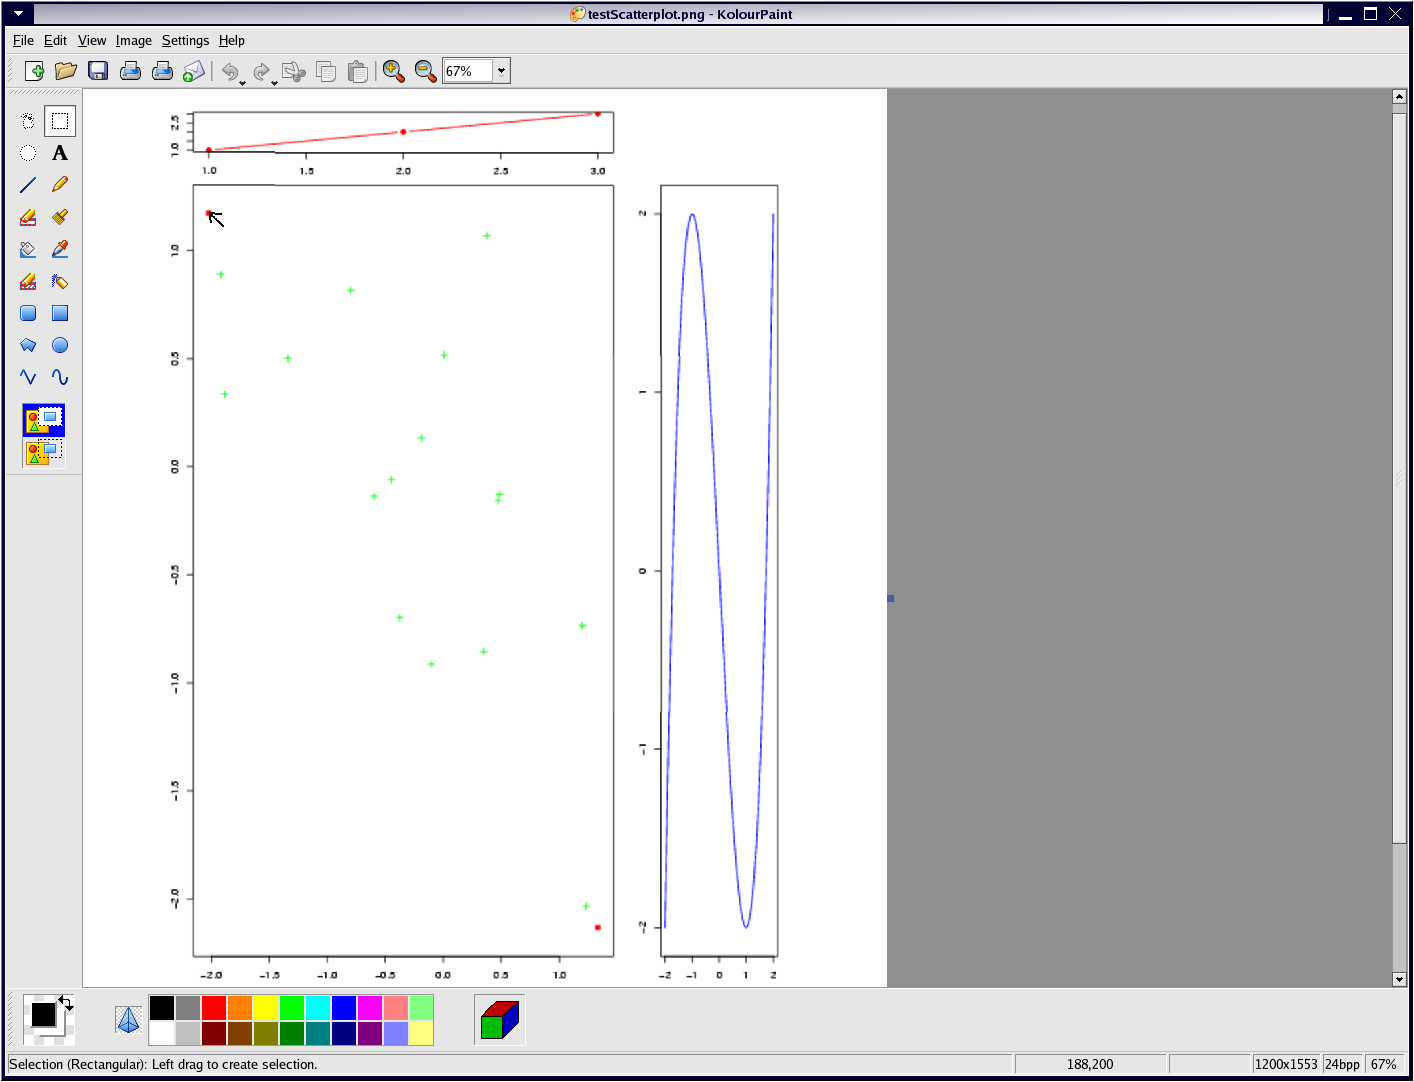
\includegraphics{sendPlot2}
\caption{scatterplot opened in kolourpaint, showing additional red points to aid in locating boundaries.Notice where pixel location can be found}
\end{figure}
\end{center}

\quad Notice the mouse is over the upper left red point for the up.left bounding box. The pixel location is shown on the bottom of the window in the second box from the left. It shows a location of 188, 200. The sendplot function used to created this figure should be rerun with bound.pt=FALSE and up.left=c(188,200). Lets look at the code that will open our example in kolourpaint. This function does not have correct up.left or low.right entries. 

\begin{verbatim}
sendplot(mat=mat, plot.calls=plot.calls, mai.mat=mai.mat,
         x=x,y=y,z=z,xlim=NA,ylim=NA, z.value=z.value, type="image",
         plt.extras=plt.extras, x.lbls=x.lbls, y.lbls=y.lbls,xy.lbls=xy.lbls, 
         spot.radius=3,up.left=c(673,715),low.right=c(2874,4481),
         source.plot=NA, img.prog=TRUE,
         resize=resize,bound.pt=TRUE, paint=TRUE)
\end{verbatim}



\begin{center}
\begin{figure}
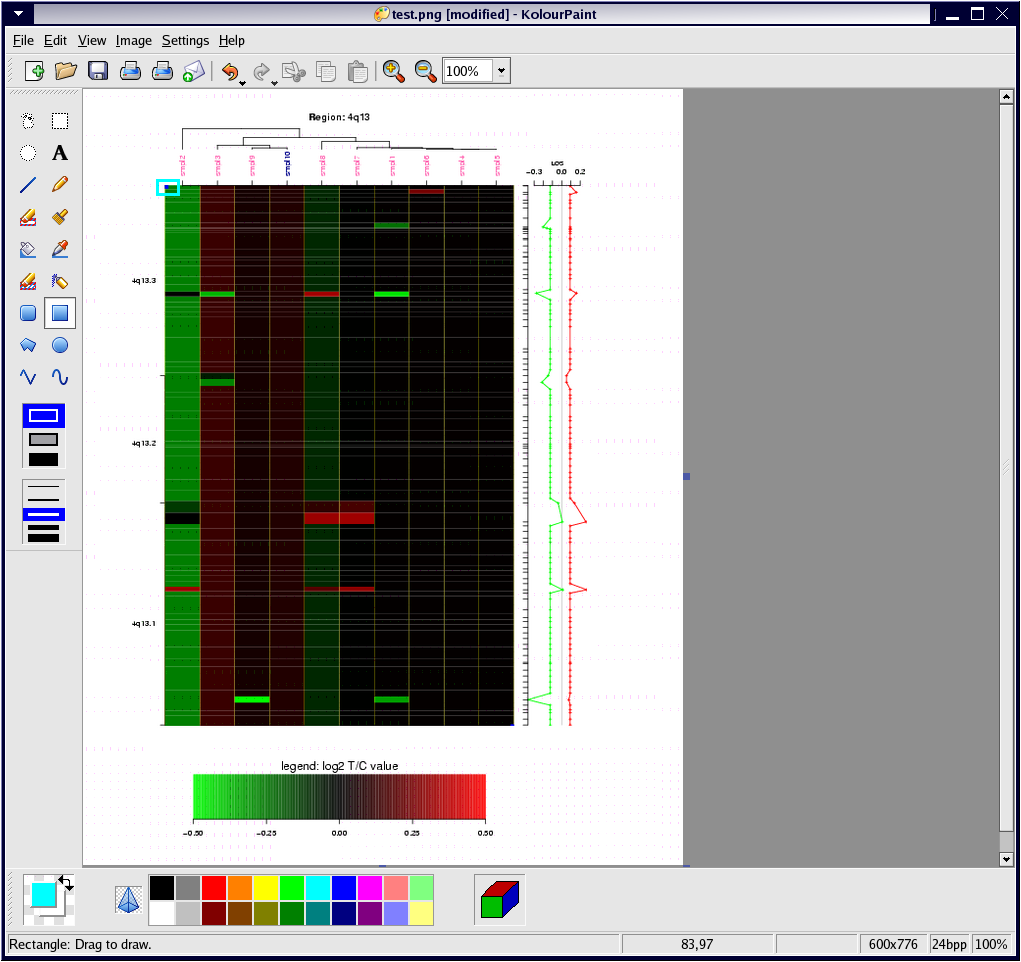
\includegraphics{sendPlot3}
\caption{our example image opened in kolourpaint. The boundaries of the image is where the pixel location should be taken.}
\end{figure}
\end{center}

\quad In Figure 6, We have circled the mouse location in blue to aid in viewing. Your mouse will not have the blue circle surrounding it. The pixel location at this location is 83,97. This therefore should be used as the up.left location. The lower right pixel location is 430, 635. After these values are determined, the sendplot function call should be run again, changing only the up.left, up.right, paint, and bound.pt argument. up.left and low.right should be updated accordingly. paint and bound.pt should be tripped to FALSE. (NOTE: these are the correct up.left and low.right boundaries when the png is created from the postscript in linux/unix environment. If the png file was generated directly, like when in a windows envirnoment, the up.left and low.right values of this example may be slightly different).  The following will make the correct interactive plot.

\begin{Schunk}
\begin{Sinput}
> sendplot(mat = mat, plot.calls = plot.calls, mai.mat = mai.mat, 
+     x = x, y = y, z = z, xlim = NA, ylim = NA, z.value = z.value, 
+     type = "image", plt.extras = plt.extras, x.lbls = x.lbls, 
+     y.lbls = y.lbls, xy.lbls = xy.lbls, spot.radius = 3, up.left = c(83, 
+         97), low.right = c(430, 635), source.plot = NA, img.prog = TRUE, 
+     resize = resize, bound.pt = FALSE, paint = FALSE)
\end{Sinput}
\end{Schunk}
\quad The resulting html file may be openned in any web browser that is capable of running javascript. We recommend using mozilla firefox; Internet Explorer currently is not supported. Figure 7 shows a snapshot of the final graph opened in firefox. Notice how the appropriate information for the region located under the white arrow is displayed in the information box.

\begin{center}
\begin{figure}
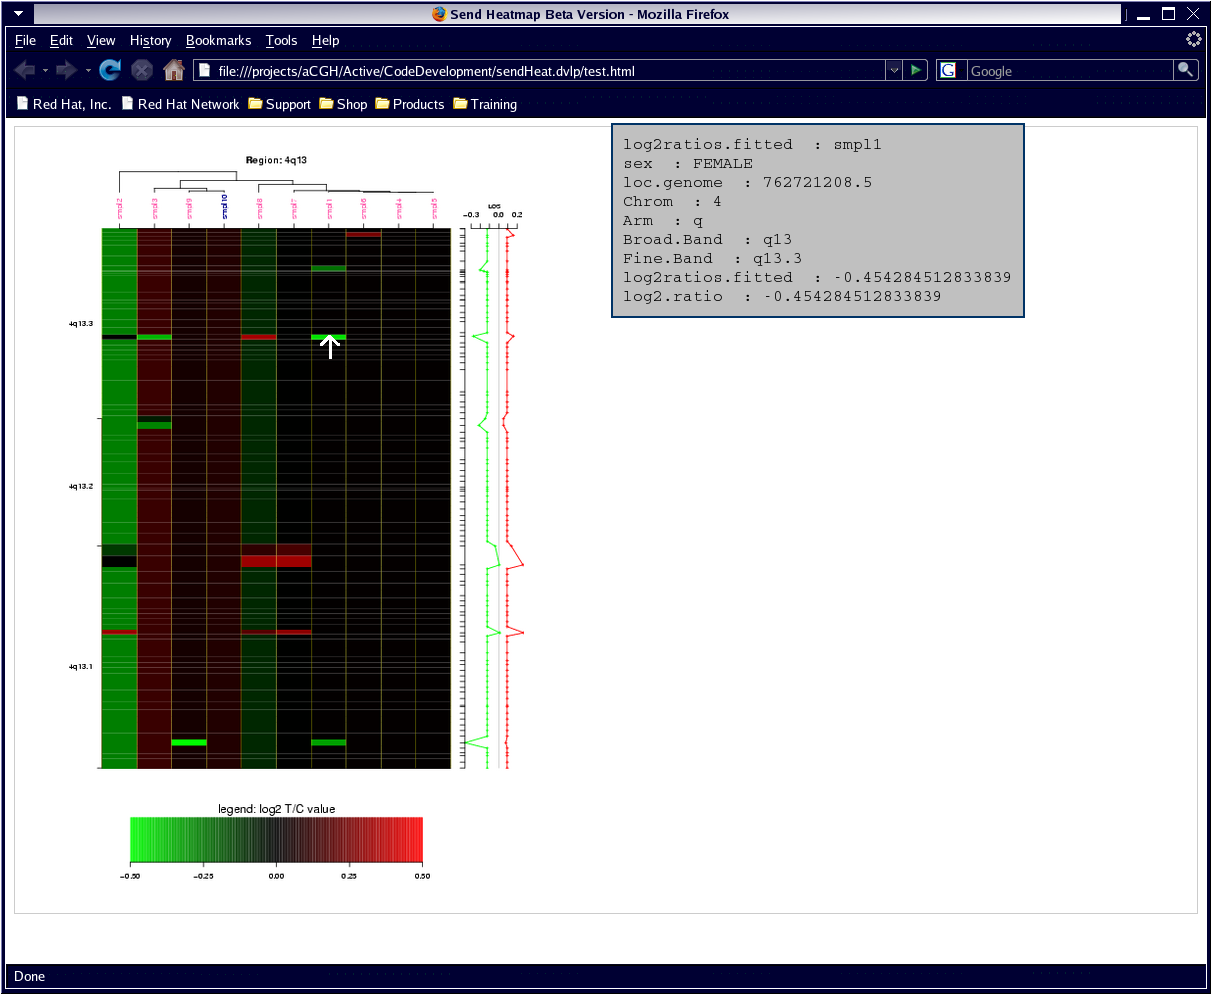
\includegraphics{sendPlot4}
\caption{snapshot of our example html file opened in firefox. The information is displayed for the region under the white arrow.}
\end{figure}
\end{center}

\quad  Briefly, the spot.radius argument controls how large an area will be active when the mouse is scrolled over. If the user selects a larger region, some spot locations may overlap and be lost. If the user selects a low region, the interactive application is very sensitive. 


\end{document}
